\section{アプローチ13（HSV色特徴抽出の撤廃とカルマンフィルタ依存の軽量化トラッキング手法）}

\subsection{手法の概要}
アプローチ12では、複数フレームにわたる時空間トラッキングとHSV色空間に基づく胴体・顔領域の色特徴量を組み合わせることで通行人の誤判定を防いだ。しかし、ピクセル単位の画像クロップや色特徴の計算・比較処理が追跡パイプライン全体のボトルネックとなり、実装の複雑化と処理負荷の増大を招いていた。

アプローチ13では、重い特徴量推定（HSV色判定）を全面的に撤廃し、カルマンフィルタによる高精度な位置推測およびバウンディングボックスの物理的移動率チェックのみに依存する軽量なトラッキング手法を検証・導入した。

本アプローチにおける簡略化および最適化仕様は以下の通りである。

\begin{itemize}
    \item \textbf{色特徴量の撤廃とデータ構造の削減}：
    \texttt{TrackedPerson} クラスおよび関連モジュールから胴体・顔領域のピクセル平均色保持ロジックを完全に削除した。これにより、毎フレームの固定サイズキャンバス経由によるクロップ画像取得処理（\texttt{imageHelper} の呼び出し）を廃止し、メモリ転送オーバーヘッドを削除した。

    \item \textbf{カルマンフィルタおよび移動割合チェックの強化}：
    特徴量による補正を排除する代わりに、カルマンフィルタ（\texttt{KalmanFilterForPeople.ts}）における状態推定精度を最適化し、バウンディングボックスのサイズに応じた移動許容範囲の動的計算ロジックを厳密化した。

    \item \textbf{滞留時間判定による連続性の維持}：
    FPS計測モジュール（\texttt{measureFps.ts}）から得られるフレームレートに基づき、バウンディングボックスの存在フレーム数および滞留時間の閾値判定のみを用いて待機列構成員と通行人の分離を実行した。
\end{itemize}

\subsection{実験結果およびアプローチ12との比較}

\subsubsection{実験結果}
静止画を入力データとして検証を行った際の実験結果を表\ref{tab:approach13_image_results}に示す。
なお、いずれの実験結果においても、緑色のバウンディングボックスは検出された人物、赤色のバウンディングボックスは同定されたグループを示している。

\begin{table}[H]
  \centering
  \small
  \caption{アプローチ13：実験結果の比較（静止画）}
  \label{tab:approach13_image_results}
  \adjustbox{max width=\textwidth}{%
  \begin{tabular}{|c|c|c|c|c|}
    
    \hline

      & \begin{tabular}{c} 前アプローチの \\ 検出結果 \end{tabular}
      & 検出結果
      & \begin{tabular}{c} 検出された \\ グループ数 \end{tabular}
      & 実際のグループ数との差 \\
    
    \hline
    
    $\vcenter{\hbox{標準状態}}$ &
      $\vcenter{\hbox{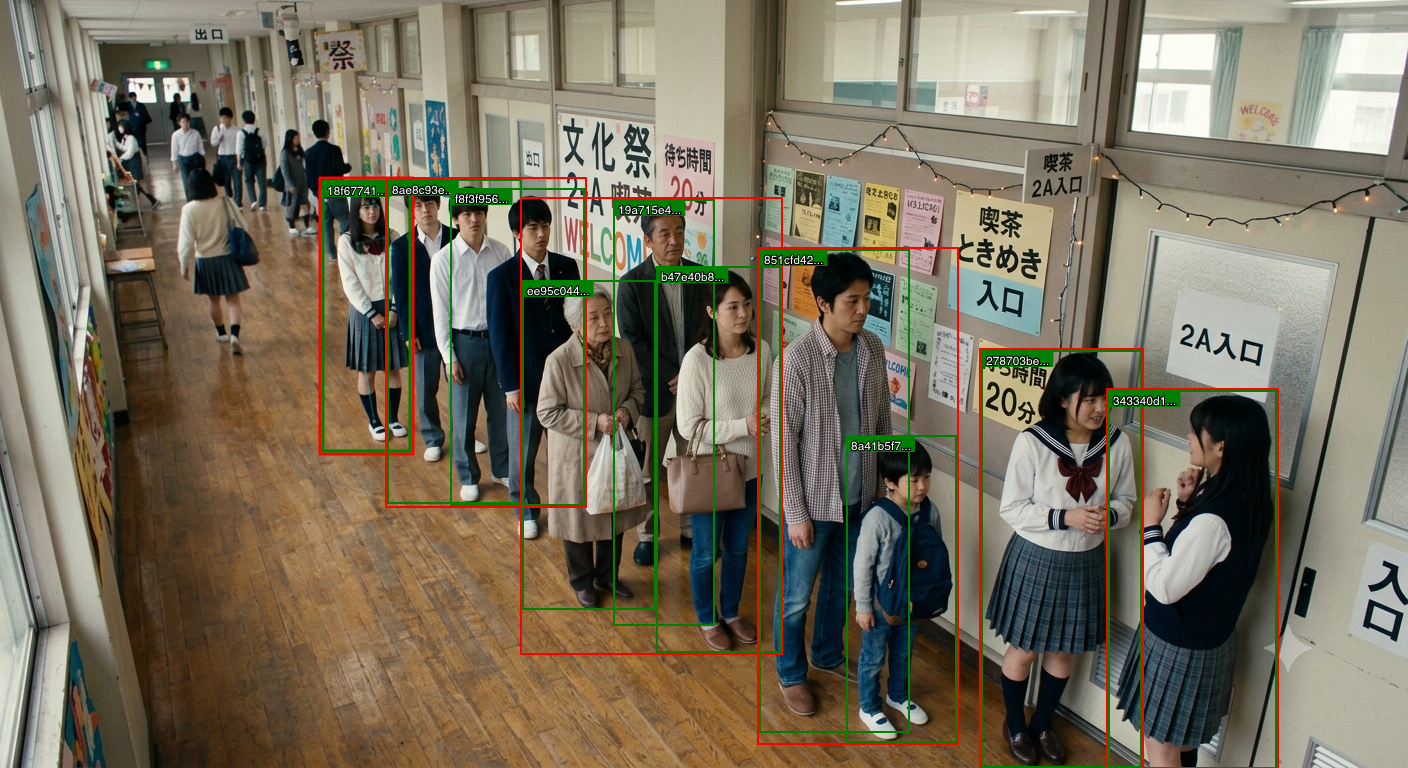
\includegraphics[width=0.25\textwidth]{experiment/results/approach_12_person_tracking/standard/detection_outputs/annotated_images/t_001s.png}}}$ &
      $\vcenter{\hbox{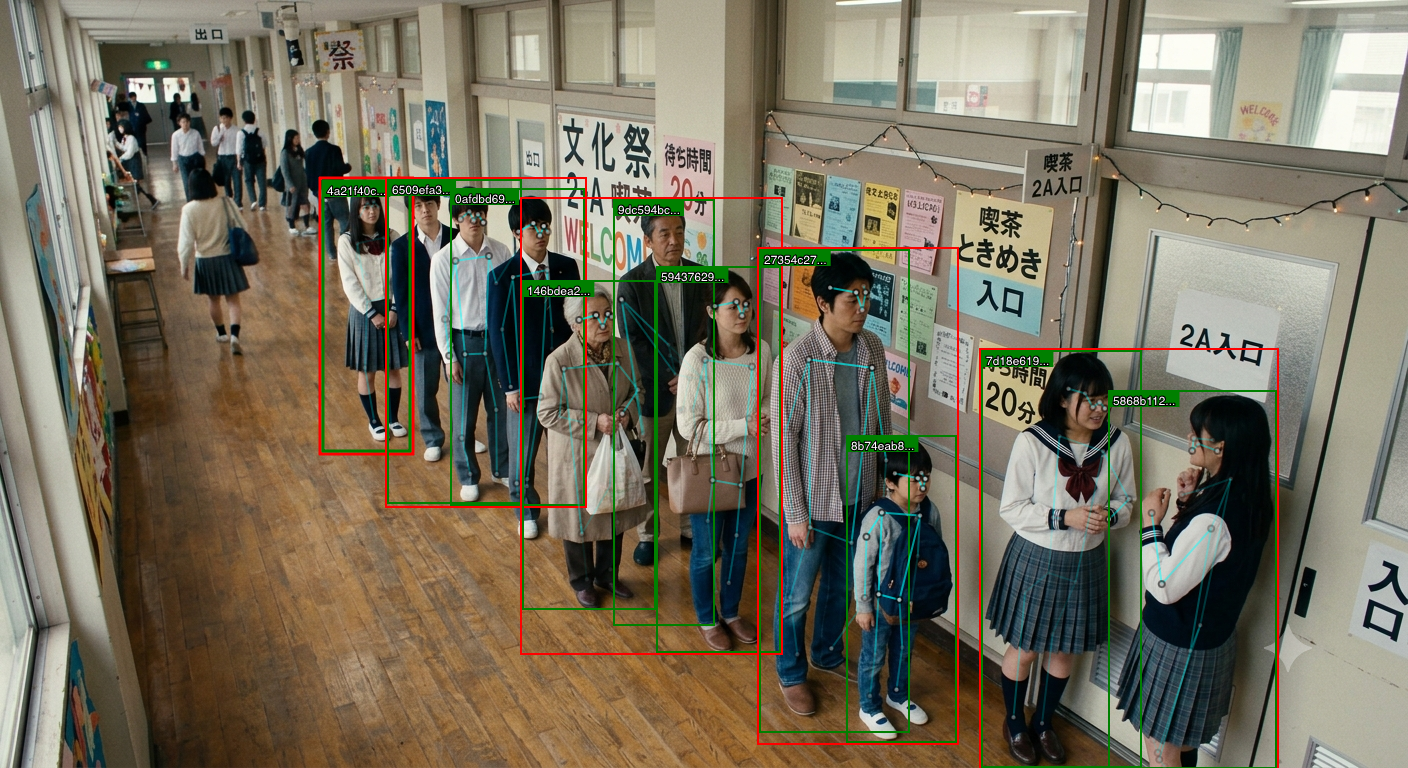
\includegraphics[width=0.25\textwidth]{experiment/results/approach_13_remove_feature_estimation/standard/detection_outputs/annotated_images/t_001s.png}}}$ &
      \jsonlen{experiment/results/approach_13_remove_feature_estimation/standard/detection_outputs/labels/t_001s.json} &
      % 符号と数値
        \ifnum\numexpr \jsonlen{experiment/results/approach_13_remove_feature_estimation/standard/detection_outputs/labels/t_001s.json} - \gtstandard\relax>0 +\fi\the\numexpr
        \jsonlen{experiment/results/approach_13_remove_feature_estimation/standard/detection_outputs/labels/t_001s.json} - \gtstandard\relax \\
    
    \hline
    
    $\vcenter{\hbox{密集状態}}$ &
      $\vcenter{\hbox{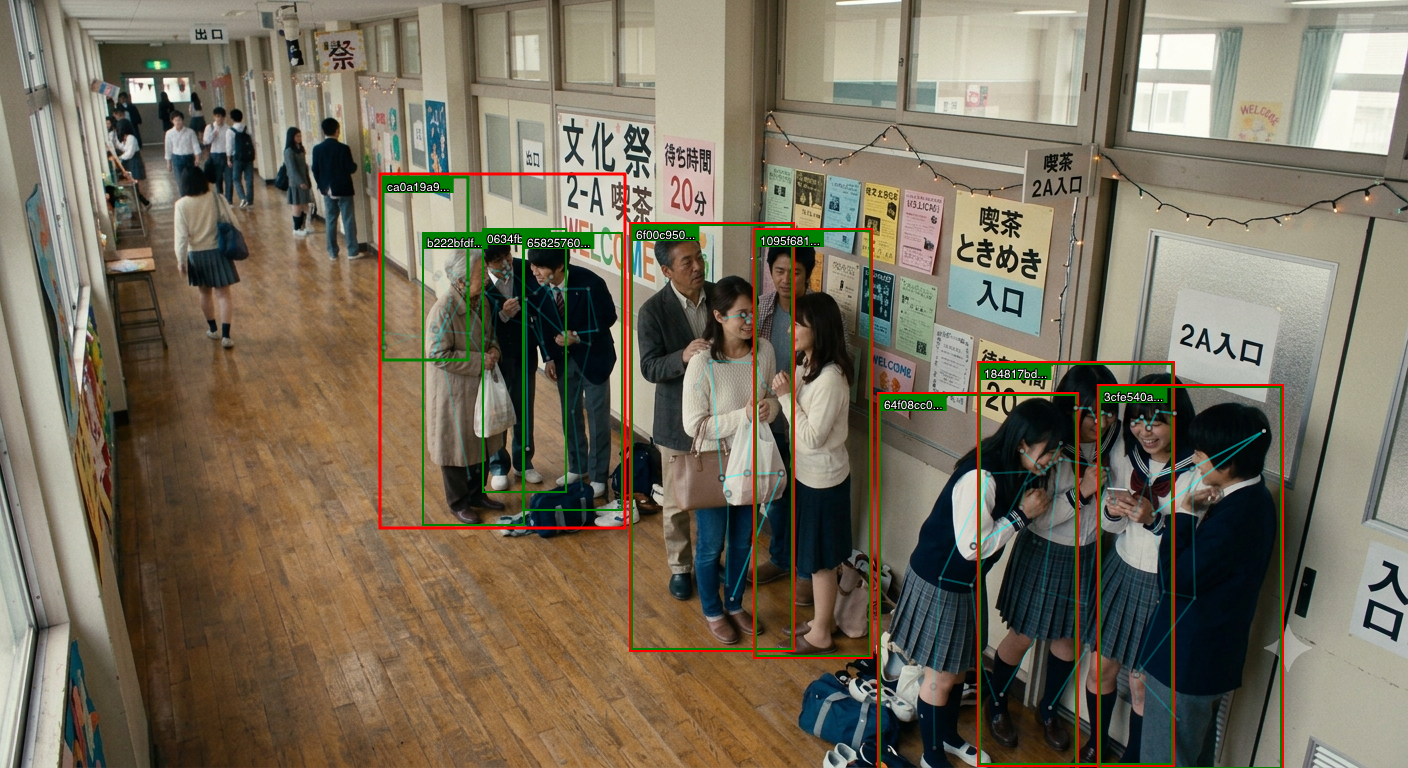
\includegraphics[width=0.25\textwidth]{experiment/results/approach_12_person_tracking/crowded/detection_outputs/annotated_images/t_001s.png}}}$ &
      $\vcenter{\hbox{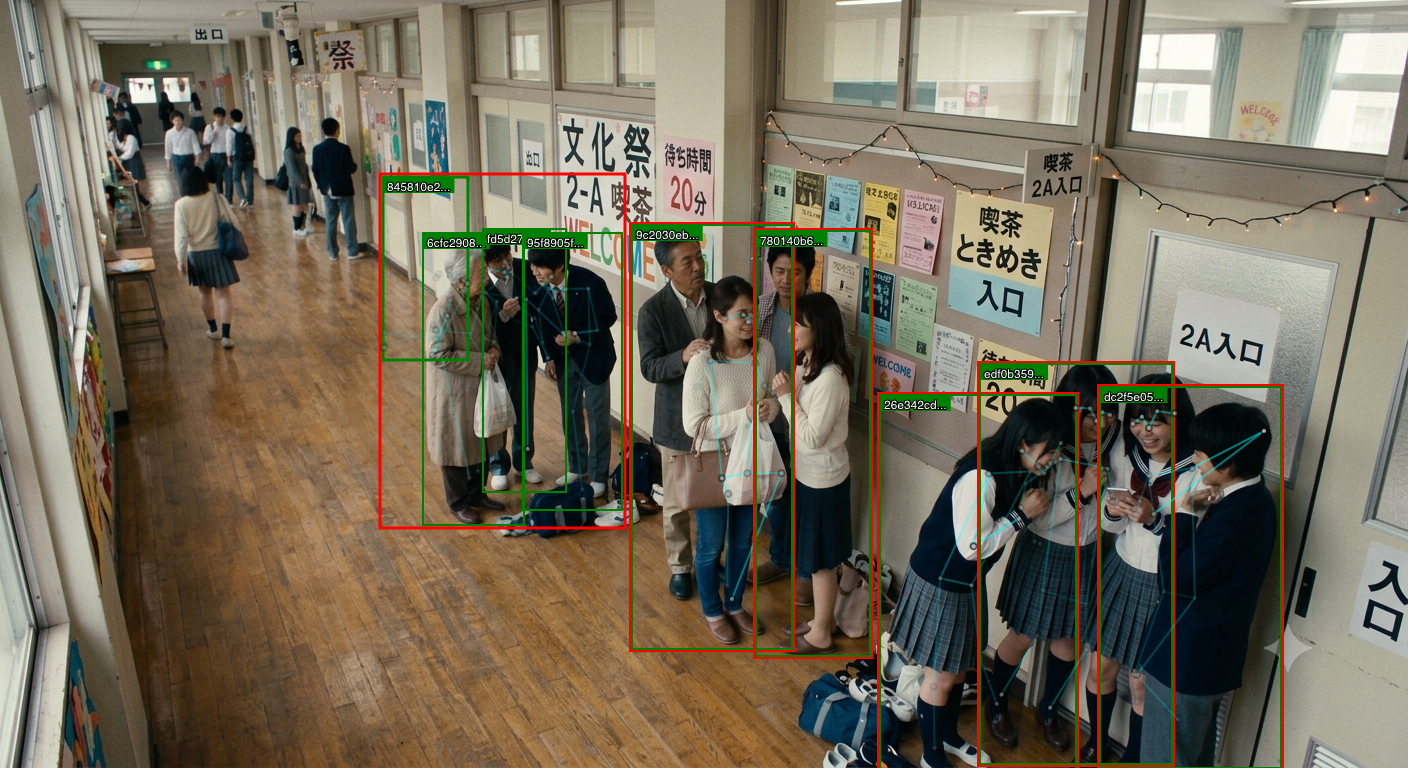
\includegraphics[width=0.25\textwidth]{experiment/results/approach_13_remove_feature_estimation/crowded/detection_outputs/annotated_images/t_001s.png}}}$ &
      \jsonlen{experiment/results/approach_13_remove_feature_estimation/crowded/detection_outputs/labels/t_001s.json} &
      % 符号と数値
        \ifnum\numexpr \jsonlen{experiment/results/approach_13_remove_feature_estimation/crowded/detection_outputs/labels/t_001s.json} - \gtcrowded\relax>0 +\fi\the\numexpr
        \jsonlen{experiment/results/approach_13_remove_feature_estimation/crowded/detection_outputs/labels/t_001s.json} - \gtcrowded\relax \\
    
    \hline
    
    $\vcenter{\hbox{非組織群集}}$ &
      $\vcenter{\hbox{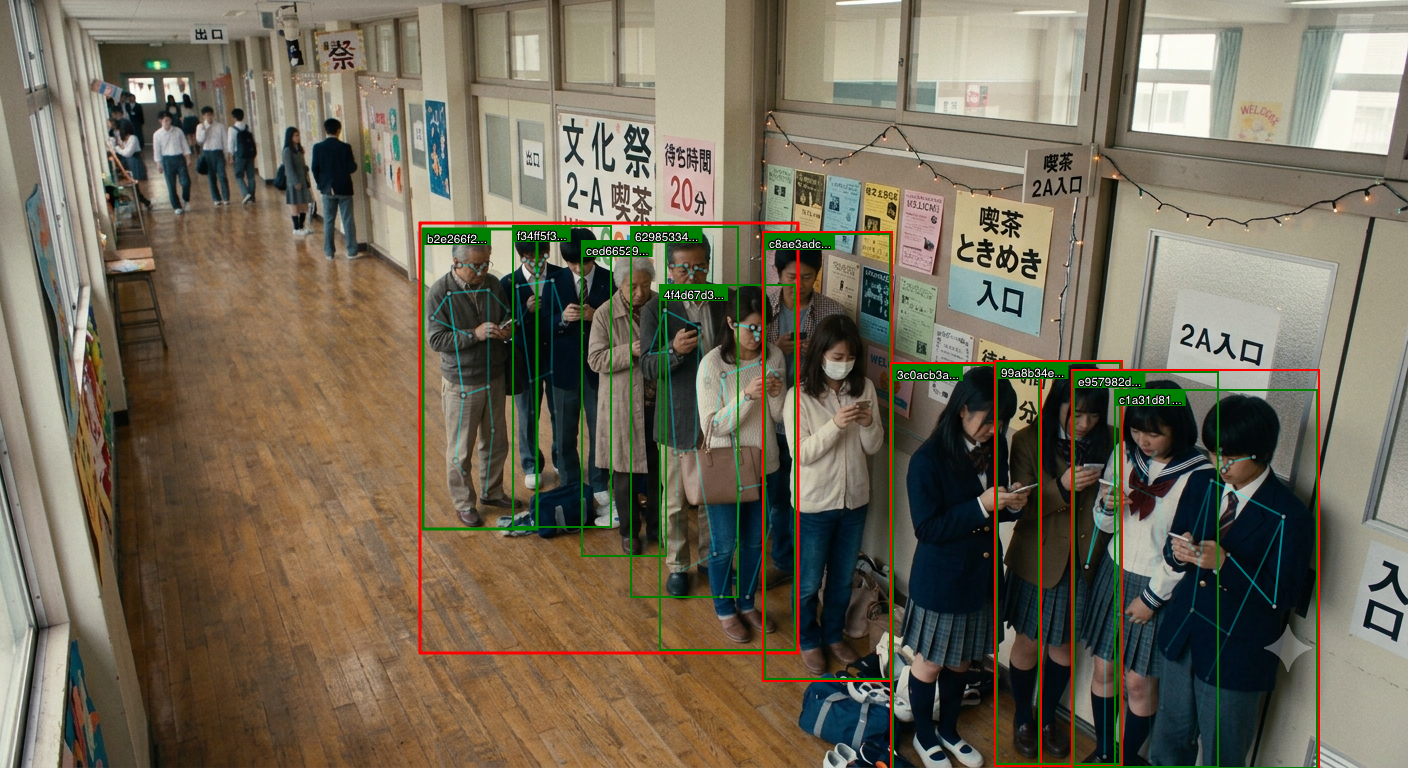
\includegraphics[width=0.25\textwidth]{experiment/results/approach_12_person_tracking/strangers/detection_outputs/annotated_images/t_001s.png}}}$ &
      $\vcenter{\hbox{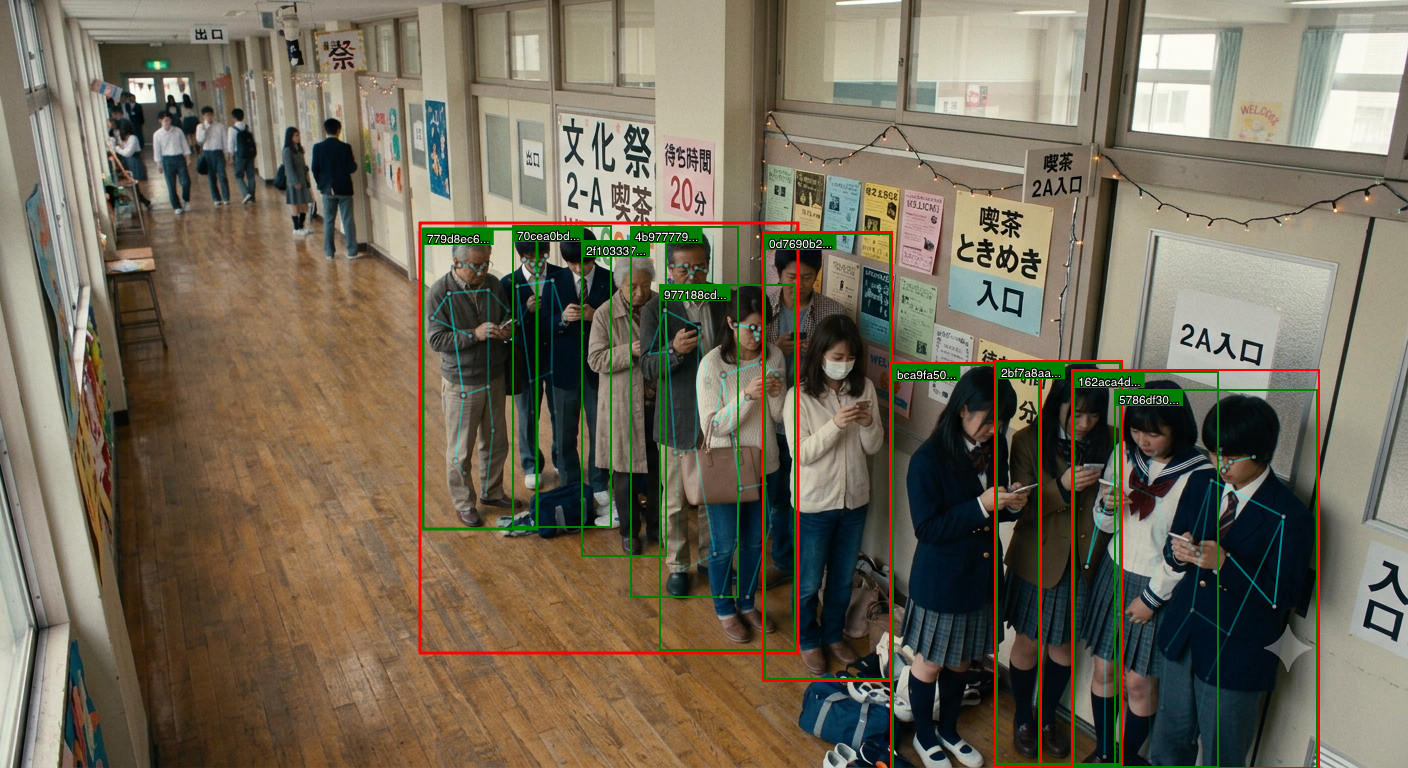
\includegraphics[width=0.25\textwidth]{experiment/results/approach_13_remove_feature_estimation/strangers/detection_outputs/annotated_images/t_001s.png}}}$ &
      \jsonlen{experiment/results/approach_13_remove_feature_estimation/strangers/detection_outputs/labels/t_001s.json} &
      % 符号と数値
        \ifnum\numexpr \jsonlen{experiment/results/approach_13_remove_feature_estimation/strangers/detection_outputs/labels/t_001s.json} - \gtstrangers\relax>0 +\fi\the\numexpr
        \jsonlen{experiment/results/approach_13_remove_feature_estimation/strangers/detection_outputs/labels/t_001s.json} - \gtstrangers\relax \\
    
    \hline
    
    $\vcenter{\hbox{視覚的クラッター}}$ &
      $\vcenter{\hbox{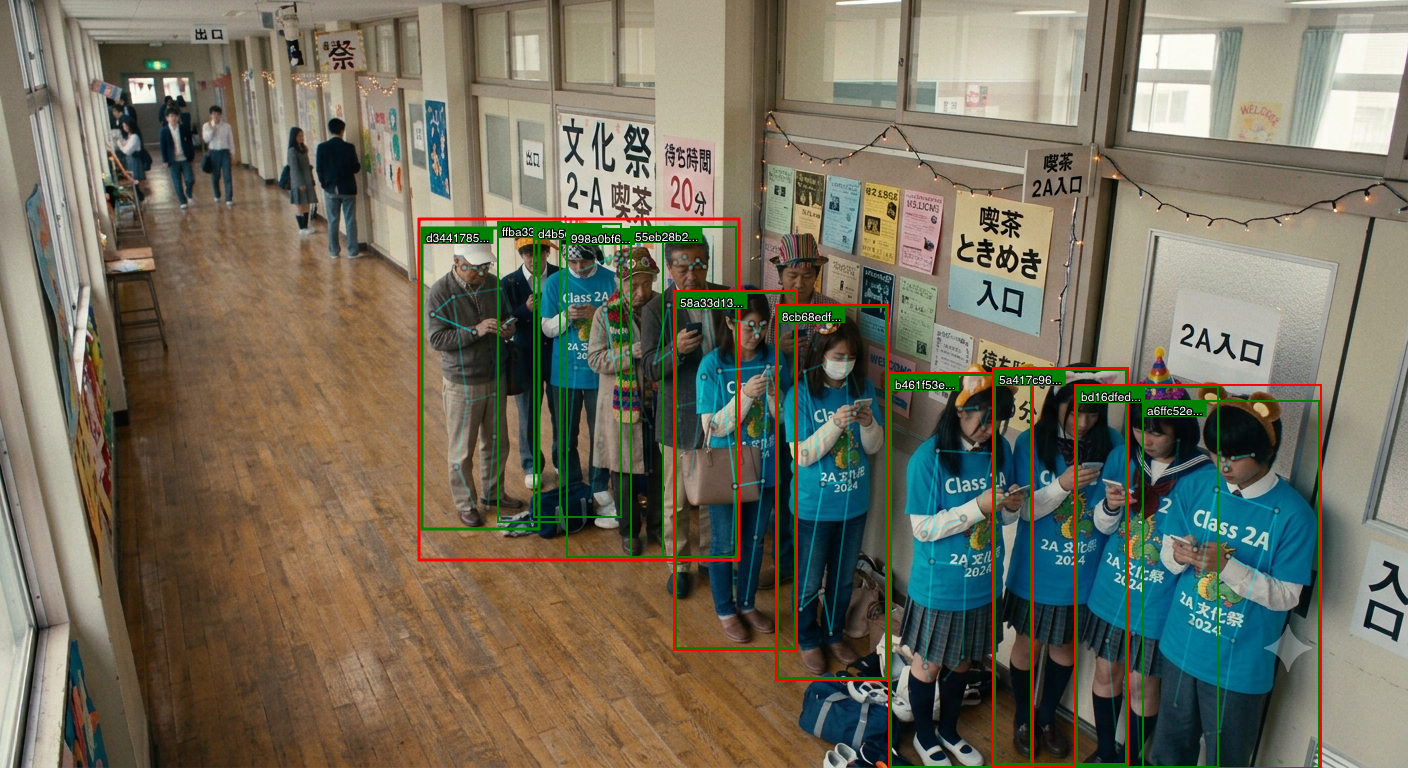
\includegraphics[width=0.25\textwidth]{experiment/results/approach_12_person_tracking/various_clothes/detection_outputs/annotated_images/t_001s.png}}}$ &
      $\vcenter{\hbox{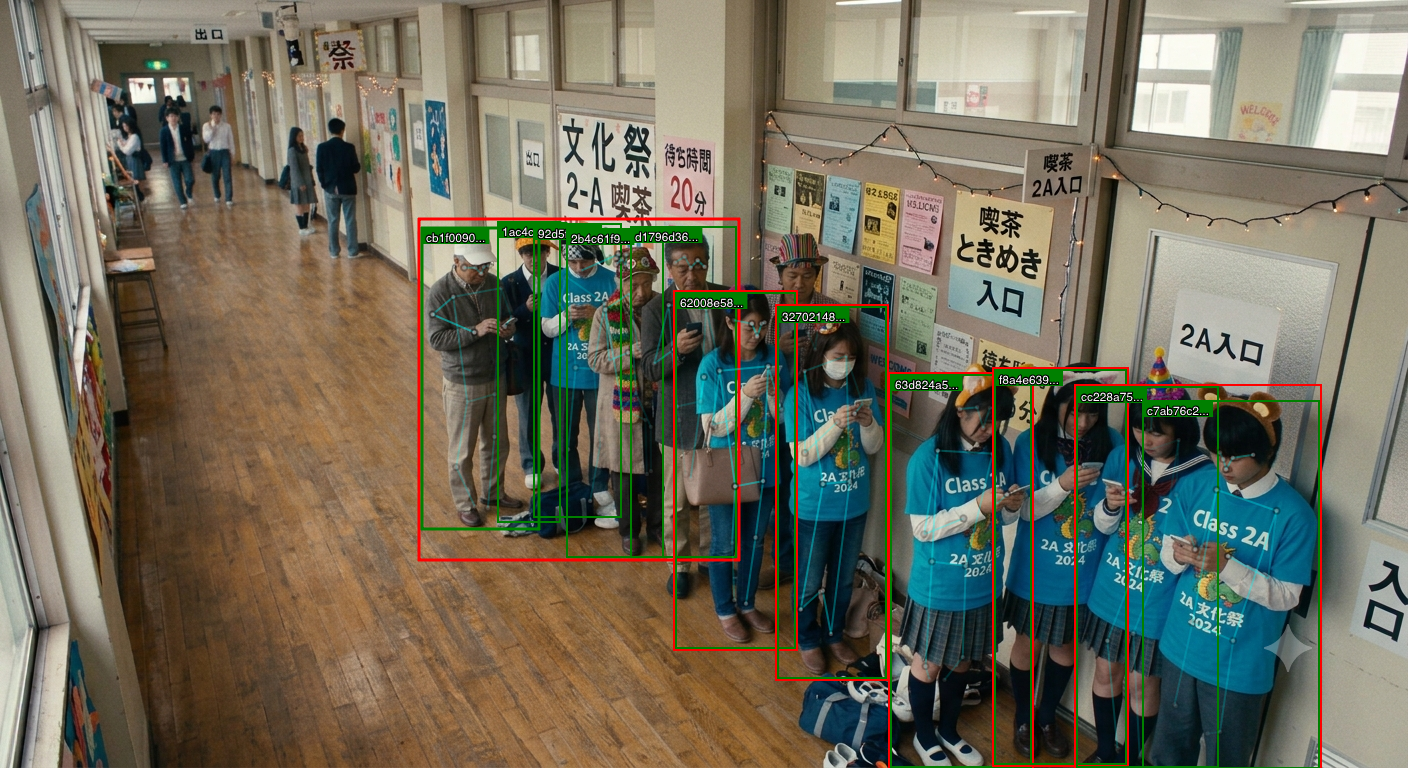
\includegraphics[width=0.25\textwidth]{experiment/results/approach_13_remove_feature_estimation/various_clothes/detection_outputs/annotated_images/t_001s.png}}}$ &
      \jsonlen{experiment/results/approach_13_remove_feature_estimation/various_clothes/detection_outputs/labels/t_001s.json} &
      % 符号と数値
        \ifnum\numexpr \jsonlen{experiment/results/approach_13_remove_feature_estimation/various_clothes/detection_outputs/labels/t_001s.json} - \gtvariousclothes\relax>0 +\fi\the\numexpr
        \jsonlen{experiment/results/approach_13_remove_feature_estimation/various_clothes/detection_outputs/labels/t_001s.json} - \gtvariousclothes\relax \\
    
    \hline

  \end{tabular}
  }
\end{table}

動画を入力データとして検証を行った際の実験結果を表\ref{tab:approach13_video_results}に示す。最も理想的な入力フレームおよびオクルージョン発生時のフレームを掲載している。

\begin{table}[H]
  \centering
  \small
  \caption{アプローチ13：実験結果の比較（動画）}
  \label{tab:approach13_video_results}
  \adjustbox{max width=\textwidth}{%
  \begin{tabular}{|c|c|c|c|c|}

    \hline

      & \begin{tabular}{c} 前アプローチの \\ 検出結果 \end{tabular}
      & 検出結果
      & \begin{tabular}{c} 検出された \\ グループ数 \end{tabular}
      & 実際のグループ数との差 \\
    
    \hline

    $\vcenter{\hbox{理想的な状態}}$ &
      $\vcenter{\hbox{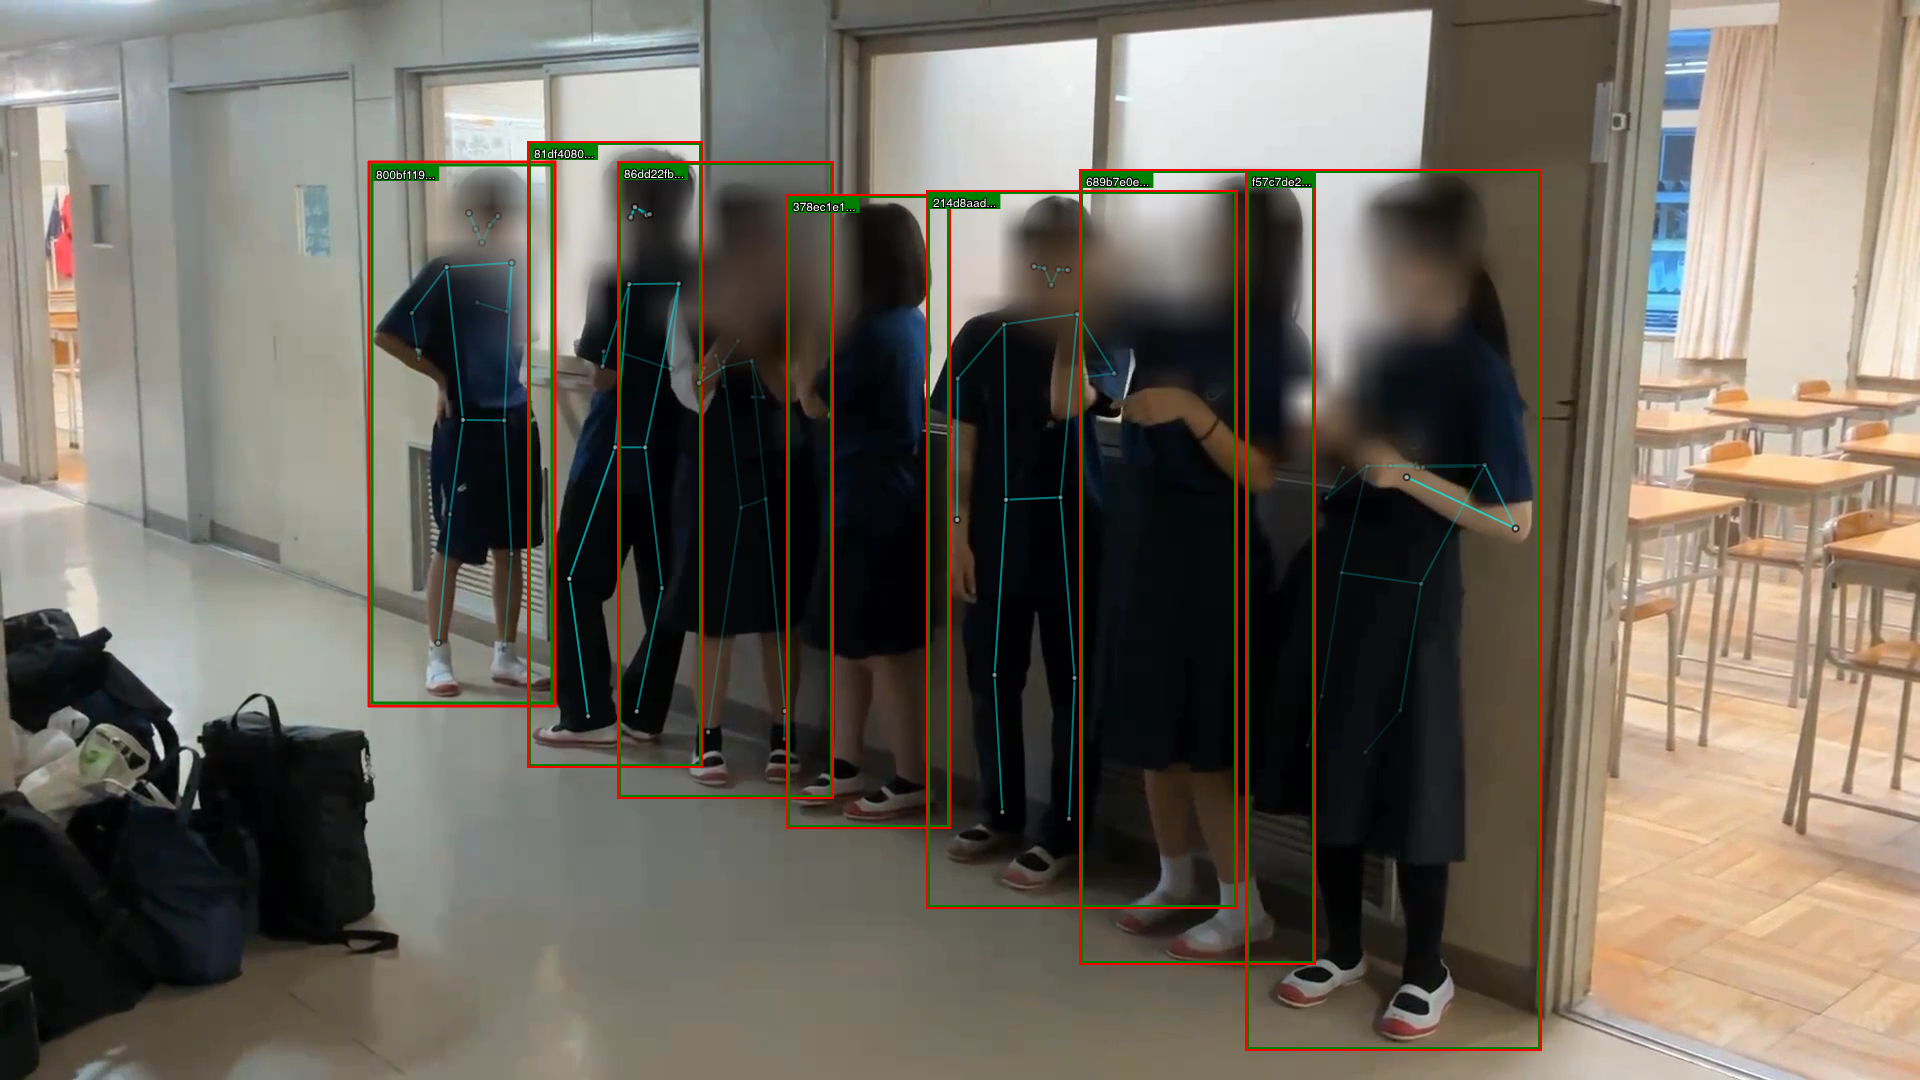
\includegraphics[width=0.25\textwidth]{experiment/results/approach_12_person_tracking/queue_video/detection_outputs/annotated_images/t_012s.png}}}$ &
      $\vcenter{\hbox{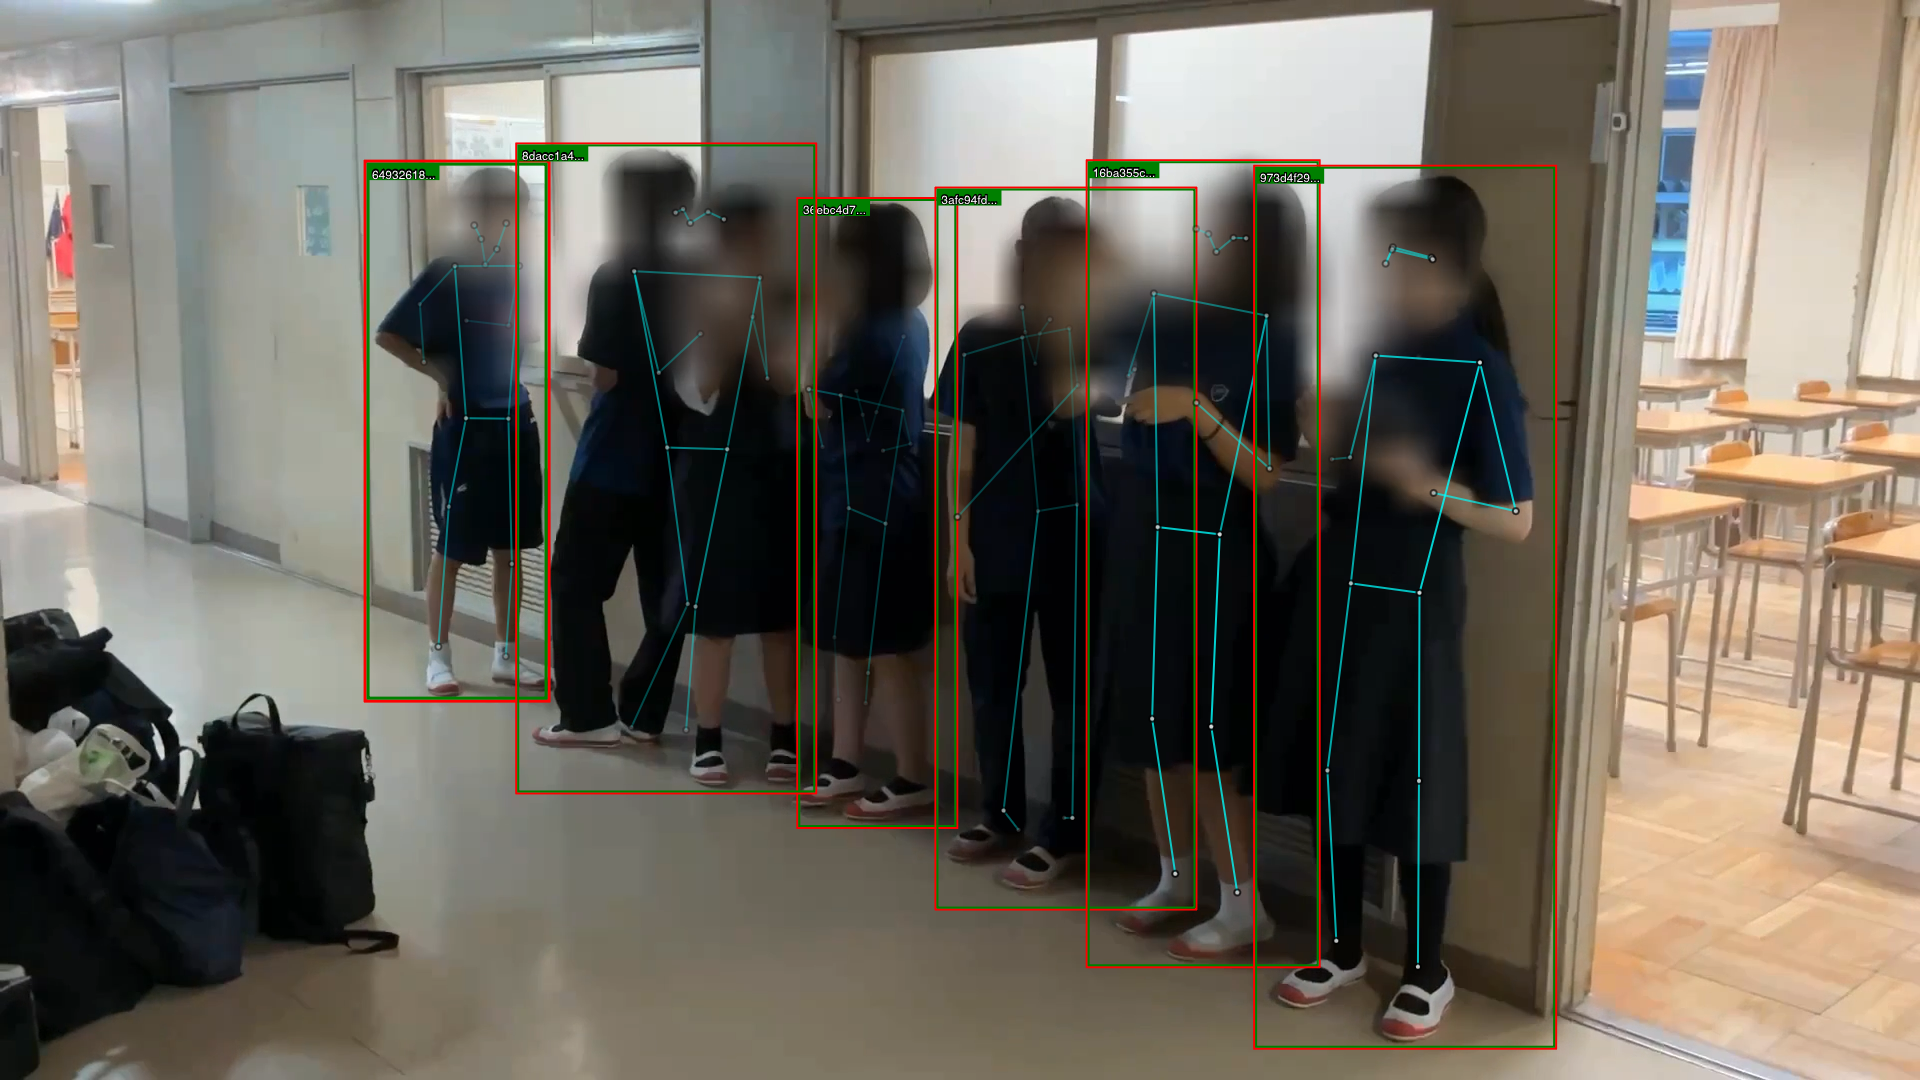
\includegraphics[width=0.25\textwidth]{experiment/results/approach_13_remove_feature_estimation/queue_video/detection_outputs/annotated_images/t_012s.png}}}$ &
      \jsonlen{experiment/results/approach_13_remove_feature_estimation/queue_video/detection_outputs/labels/t_012s.json} &
      % 符号と数値
        \ifnum\numexpr\jsonlen{experiment/results/approach_13_remove_feature_estimation/queue_video/detection_outputs/labels/t_012s.json} - \gtvideoideal\relax>0 +\fi\the\numexpr
        \jsonlen{experiment/results/approach_13_remove_feature_estimation/queue_video/detection_outputs/labels/t_012s.json} - \gtvideoideal\relax \\
    
    \hline
    
    $\vcenter{\hbox{オクルージョン発生時}}$ &
      $\vcenter{\hbox{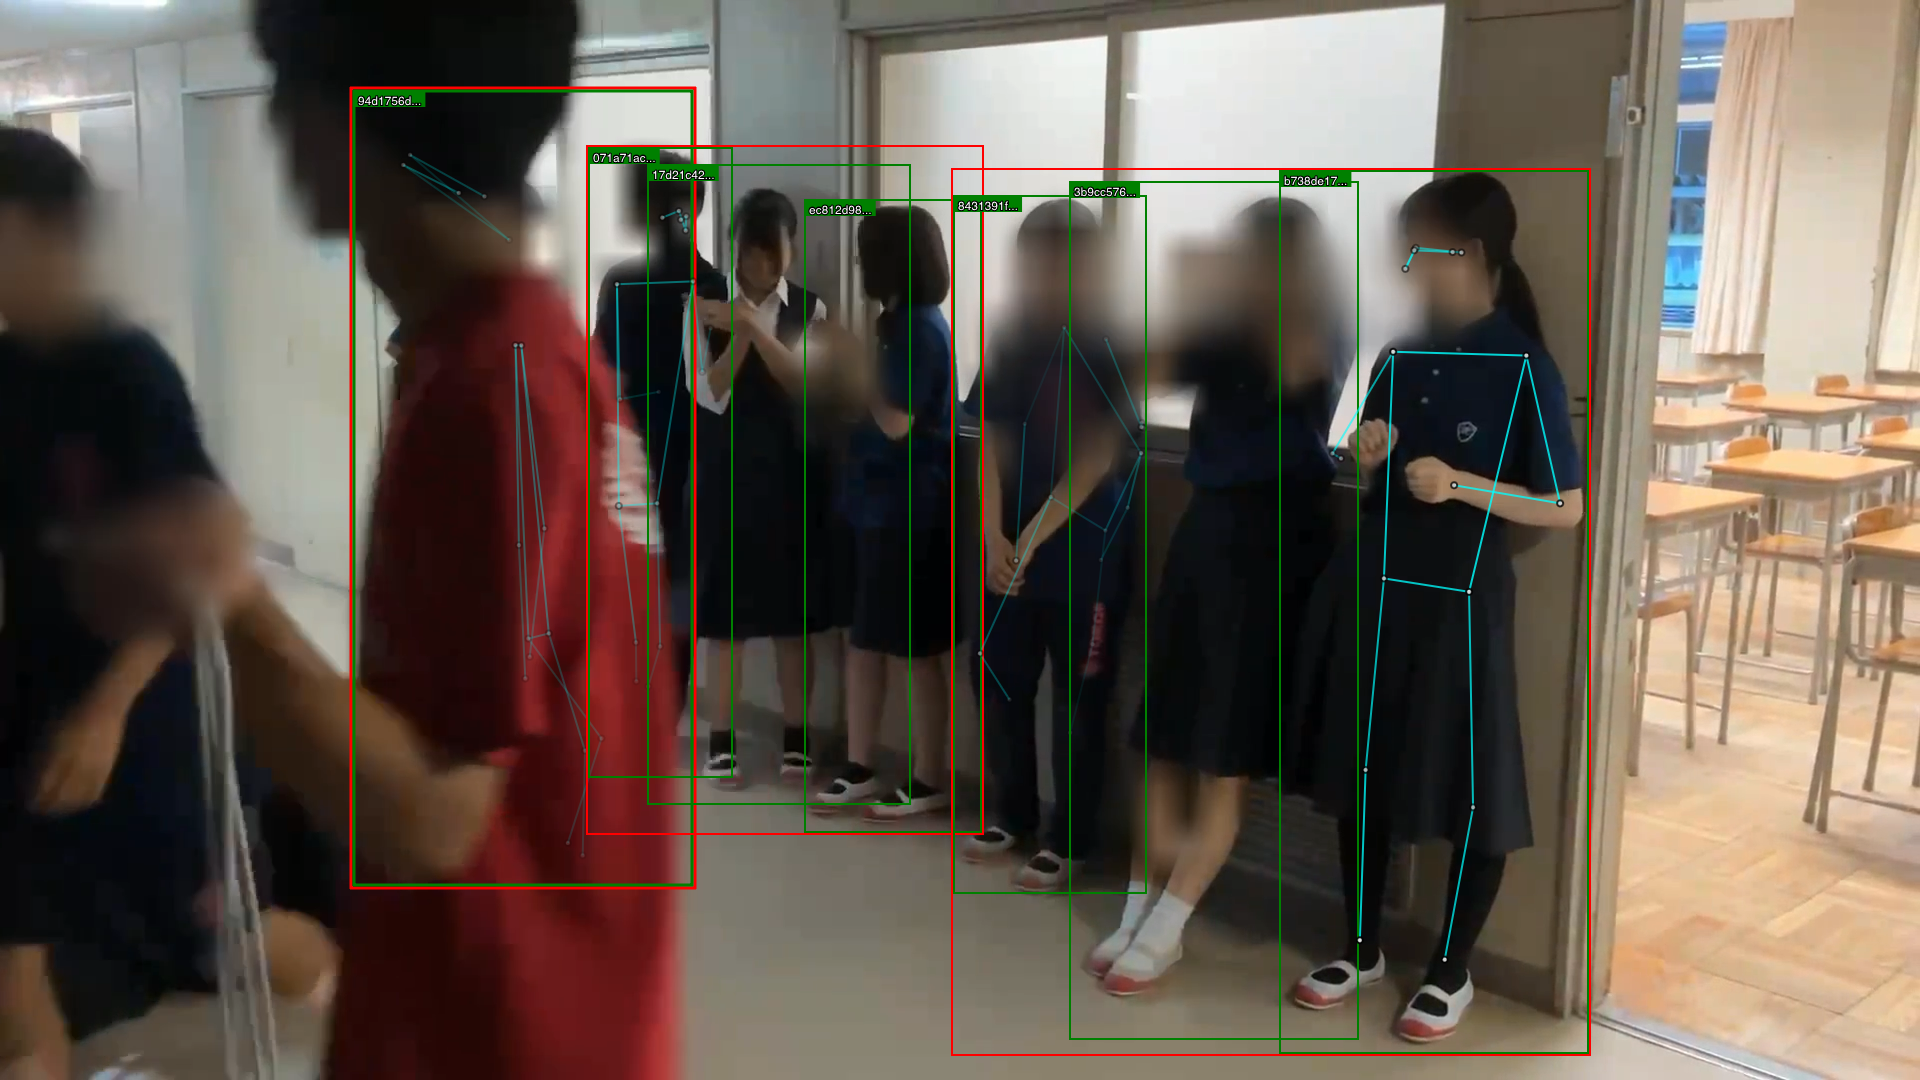
\includegraphics[width=0.25\textwidth]{experiment/results/approach_12_person_tracking/queue_video/detection_outputs/annotated_images/t_017s.png}}}$ &
      $\vcenter{\hbox{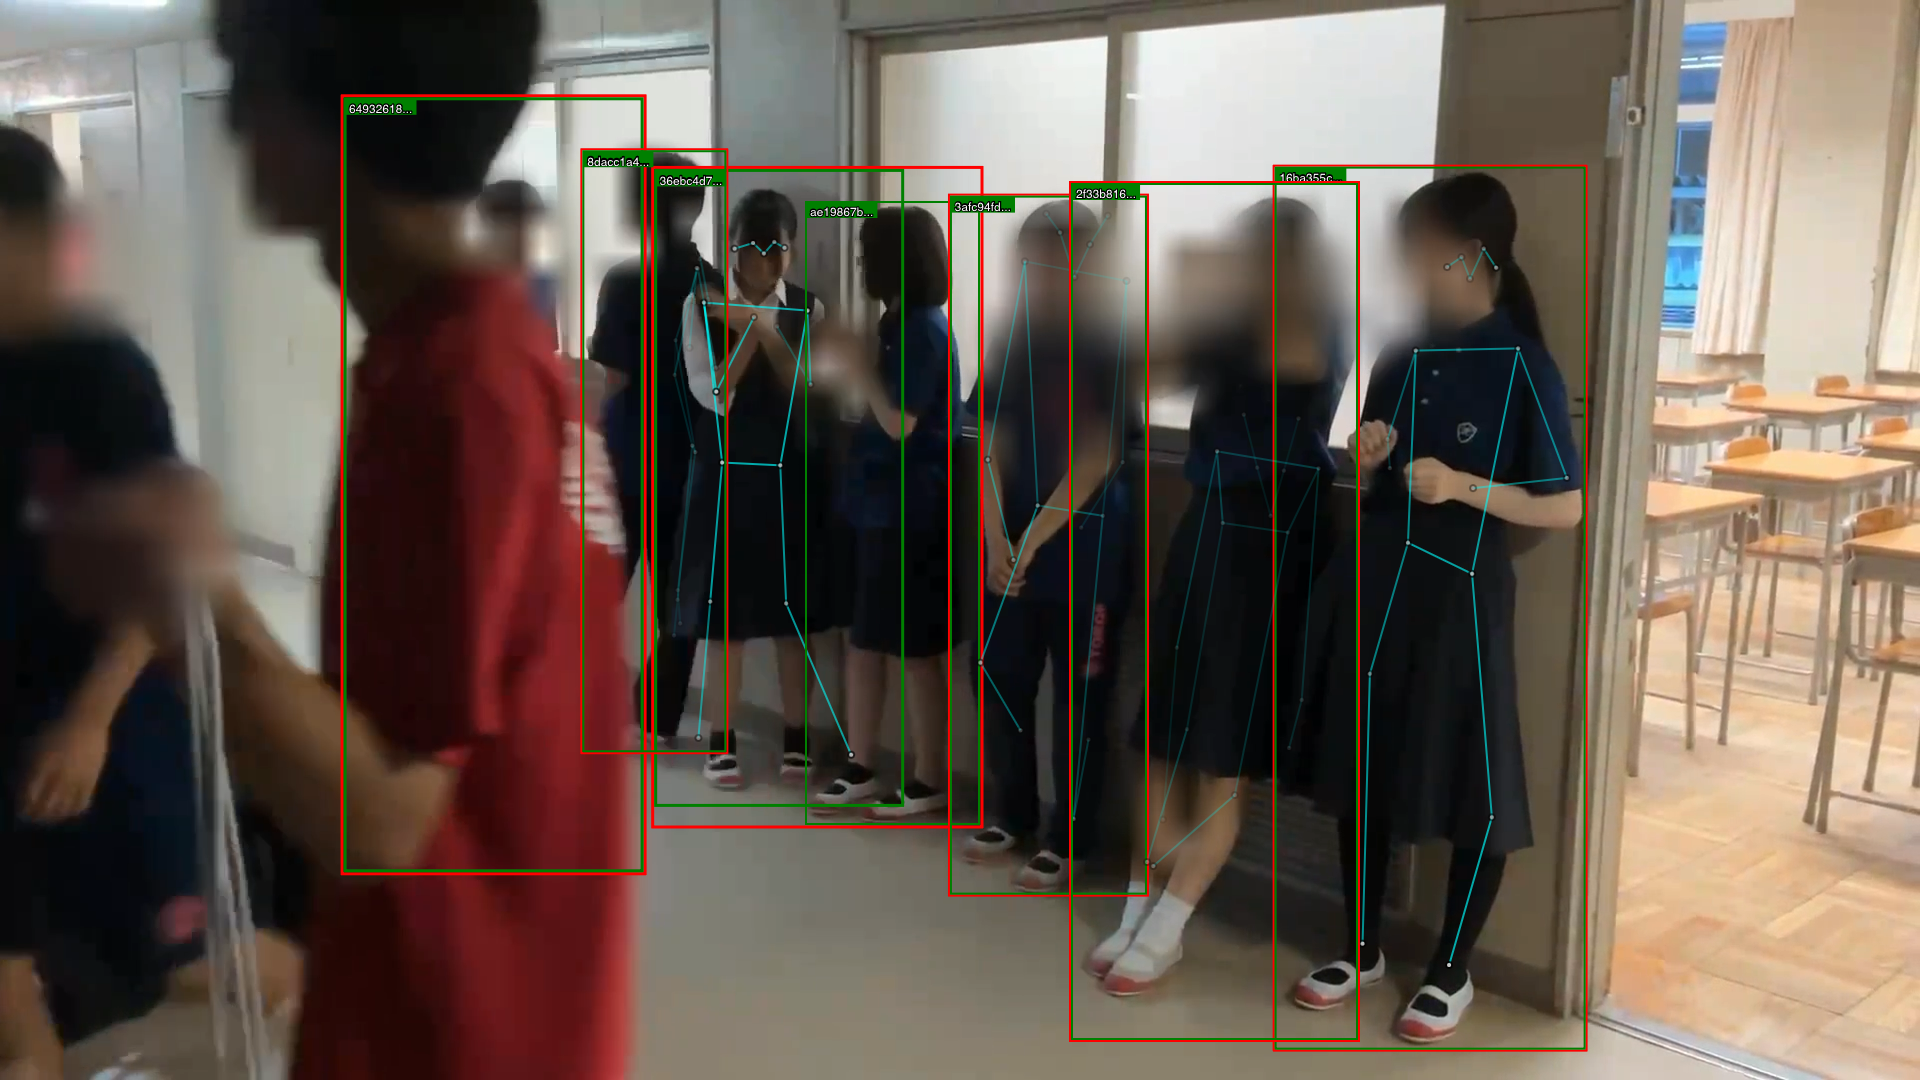
\includegraphics[width=0.25\textwidth]{experiment/results/approach_13_remove_feature_estimation/queue_video/detection_outputs/annotated_images/t_017s.png}}}$ &
      \jsonlen{experiment/results/approach_13_remove_feature_estimation/queue_video/detection_outputs/labels/t_017s.json} &
      % 符号と数値
        \ifnum\numexpr\jsonlen{experiment/results/approach_13_remove_feature_estimation/queue_video/detection_outputs/labels/t_017s.json} - \gtvideoocclusion\relax>0 +\fi\the\numexpr
        \jsonlen{experiment/results/approach_13_remove_feature_estimation/queue_video/detection_outputs/labels/t_017s.json} - \gtvideoocclusion\relax \\
    
    \hline
    
  \end{tabular}%
  }
\end{table}

\subsubsection{アプローチ12との比較}
HSV色特徴量の抽出処理を撤廃したことで、追跡ステップにおける計算負荷が大幅に軽減され、フレームレートの向上が達成された。実験の結果、十分な滞留時間閾値とカルマンフィルタによるスムーズな座標補正を組み合わせることで、複雑な色特徴を用いずとも通行人の一時的な通過を誤検出することなく排除可能であることが実証された。

\clearpage % 視認性のために改ページ挿入
